\section{Exploratory Extension: An Adaptive Down Threshold}
\label{app:adaptive}

This appendix supports Section~\ref{subsec:rq3}. The extension is exploratory, and its results do not support claiming it as a contribution.

\textbf{Exploratory extension: an adaptive down threshold.} A static threshold
trades reaction time against noise immunity, and the right point depends on
network conditions that change over time. This appendix evaluates an
extension that tries to follow them. We report it as exploratory and do not claim
it as a contribution; the summary at its end gives the reason. We extend the backoff already used on
\textsc{Recovering} to the down threshold $k_{\downarrow}$ of both demotion
edges (Section~\ref{subsec:transitions}). The effective threshold is
$k_{\downarrow} = \min(k_{\max},\, k_0 \cdot 2^{c})$, where the flap level $c$
rises by one at each such demotion and falls by one after $T_{\text{stable}}$
healthy \textsc{Anchored} blocks. $k_{\downarrow}$ depends only on committed
state, so it remains deterministic across validators. It starts at the
responsive value $k_0$ and rises only when the network proves noisy, which
also raises the cost of the repeated-trigger attack discussed in
Section~\ref{sec:discussion}. The mechanism is implemented in the
specification and in the prototype.
We swept the down threshold live on the seven-validator cluster
(Table~\ref{tab:adaptive-live}): static $k\in\{2,4,6,8\}$, each its own cap, and
the adaptive threshold ($k_0{=}2$, $k_{\max}{=}8$), under wide-area latency
jitter with no fault, under DA blips (all seven bridges stopped and restored
in cycles of tens of seconds), and under a sustained DA outage (all bridges
stopped) to measure detection. All 33
runs completed. A static value keeps no hidden state, so one genesis served all
its trials and environments; the adaptive configuration was redeployed for every
run because its flap level lives on the chain. Static $k{=}2$, $k{=}6$ and the
adaptive threshold have three trials each; $k{=}4$ and $k{=}8$ have one.

\begin{table}[h]
\caption{Live down-edge sweep on seven validators (300\,s runs, mean $\pm$
95\% Student-$t$ interval over the runs, none for a single run; flaps and uptime
averaged over the seven validators of a trial). ``Uptime'' is the share of the
run in \textsc{Anchored}; ``Detection'' is the delay from stopping the bridges of the sustained outage
to the first non-\textsc{Anchored} state on one validator, and ``To
\textsc{Sovereign}'' the delay to \textsc{Sovereign}.}
\label{tab:adaptive-live}
\centering
\footnotesize
\resizebox{\linewidth}{!}{\begin{tabular}{@{}lrrrrrr@{}}
\toprule
\textbf{Configuration} & \textbf{$n$} & \textbf{Flaps (WAN)} & \textbf{Uptime (WAN, \%)} & \textbf{Uptime (DA blips, \%)} & \textbf{Detection (s)} & \textbf{To \textsc{Sovereign} (s)} \\
\midrule
static $k{=}2$ & 3 & 9.0 $\pm$ 0.0 & 82 $\pm$ 3 & 1 $\pm$ 0 & 9.4 $\pm$ 0.4 & 38 $\pm$ 2 \\
static $k{=}4$ & 1 & 0.0 & 100 & 1 & 11.1 & 41 \\
static $k{=}6$ & 3 & 0.0 $\pm$ 0.0 & 100 $\pm$ 0 & 2 $\pm$ 2 & 12.8 $\pm$ 3.2 & 44 $\pm$ 5 \\
static $k{=}8$ & 1 & 0.0 & 100 & 3 & 14.6 & 43 \\
adaptive ($2\to8$) & 3 & 8.3 $\pm$ 2.9 & 85 $\pm$ 7 & 1 $\pm$ 0 & 11.7 $\pm$ 0.9 & 42 $\pm$ 3 \\
\bottomrule
\end{tabular}
}
\end{table}

Under jitter alone the static default of 2 flapped nine times per validator and
spent 82\% of the run in \textsc{Anchored}, and every static value from 4 up
held \textsc{Anchored} without a flap. The adaptive threshold did not behave
like the larger values: 8.3 flaps and 85\% uptime, within the interval of
$k{=}2$. Under DA blips no configuration stayed in \textsc{Anchored} (1--3\%
uptime), so the threshold did not matter there. Detection delay grew with the
threshold, from 9.4\,s at $k{=}2$ to 14.6\,s at $k{=}8$ (one run), and the
adaptive configuration sat between $k{=}2$ and $k{=}6$ at 11.7\,s. In this
sweep the adaptive threshold therefore bought no flap suppression over a static
$k{=}2$, whereas a static $k$ of 4 or more suppressed all flapping at a cost of
under 2\,s of detection delay for $k{=}4$; with one trial at $k{=}4$ and
$k{=}8$ this is an observation, not an estimate. We did not measure the
cost the adaptive threshold imposes on a repeated-trigger attacker, which is
its stated purpose. A longer stable window is a candidate explanation for the
weak suppression, since the flap level decays after 16 healthy blocks, about
twenty seconds. We therefore repeated the adaptive configuration with a window
of 64 blocks, under jitter and under the sustained outage only, three runs each,
every run on a fresh genesis (last row of Table~\ref{tab:adaptive-live}). Flaps
fell from 8.3 to 3.0 per validator (all three runs gave 3), uptime rose from 85
to 93\%, and the detection delay did not change (11.1 against 11.7\,s). A
window of 64 blocks recovers part of the gap, but not the full suppression of a
static $k$ of 4 or more; we did not test larger windows or the DA-blip
environment with it.

\textbf{Changing noise and a repeated-trigger adversary (simulation).} The sweep
above holds the noise constant, the case in which a well-chosen static
threshold needs no adaptation. The case for the adaptive threshold is noise
that changes, and a party that triggers demotions on purpose. We tested both
in-process with the keeper's own transition code. Noise is a sequence of
bursts of one to three consecutive warning-level blocks, each starting with
probability 0.03 per block; this reproduces the live demotion rate of a static
threshold of 2 (4.6 demotions per 250 blocks, against 5.0 per 300\,s live),
and the same 200 noise schedules drive every configuration, so differences are
paired. A run has 150 quiet blocks, 250 noisy blocks and a quiet phase, after
which a sustained DA outage starts and we count the blocks until the first
non-\textsc{Anchored} state. The adversary sends warning-level bursts for 1200
blocks and waits for \textsc{Anchored} between them: a naive one always sends
$k_0$ blocks with one healthy block in between, a patient one waits for the flap
level to return to zero first. The last column of Table~\ref{tab:adaptive-sim} is the concealment
simulation of Section~\ref{sec:discussion}.

\begin{table}[h]
\caption{Static and adaptive down thresholds in the in-process simulation
(blocks; mean $\pm$ 95\% interval over 200 paired noise schedules). ``Detect
after noise'' starts the outage as soon as the chain is \textsc{Anchored}
again. Repeated trigger: demotions in 1200 blocks. Outage hidden: placements
out of 35 of three Byzantine proposers that keep a real DA outage from being
detected, with the chain quiet and with the flap level at its highest.}
\label{tab:adaptive-sim}
\centering
\footnotesize
\resizebox{\linewidth}{!}{\begin{tabular}{@{}lrrrrrr@{}}
\toprule
 & \multicolumn{3}{c}{\textbf{Changing noise}} & \multicolumn{2}{c}{\textbf{Repeated trigger}} & \textbf{Outage hidden} \\
\cmidrule(lr){2-4}\cmidrule(lr){5-6}
\textbf{Threshold} & \textbf{Detect, quiet} & \textbf{Flaps} & \textbf{Detect after noise} & \textbf{Naive} & \textbf{Patient} & \textbf{quiet / raised} \\
\midrule
static $k{=}2$ & 2.0 $\pm$ 0.0 & 8.2 $\pm$ 0.5 & 2.0 $\pm$ 0.0 & 300 & 300 & 0\,/\,0 \\
static $k{=}4$ & 4.0 $\pm$ 0.0 & 0.2 $\pm$ 0.1 & 3.9 $\pm$ 0.1 & 200 & 200 & 28\,/\,28 \\
adaptive $2\to8$, $T_{\text{stable}}{=}64$ & 2.0 $\pm$ 0.0 & 3.4 $\pm$ 0.2 & 3.2 $\pm$ 0.2 & 1 & 18 & 0\,/\,35 \\
adaptive $2\to4$, $T_{\text{stable}}{=}64$ & 2.0 $\pm$ 0.0 & 3.4 $\pm$ 0.2 & 3.1 $\pm$ 0.1 & 1 & 18 & 0\,/\,28 \\
\bottomrule
\end{tabular}
}
\end{table}

Against a static threshold of 2, the adaptive one detects the outage as fast
when the network is quiet (2 blocks), cuts the flaps of the noisy phase from 8.2
to 3.4, and absorbs the naive adversary (1 demotion against 300); a patient
adversary obtains 18. Against a static threshold of 4 it does not win on flaps
(3.4 against 0.2). What it keeps is the 2-block detection when quiet, about two
seconds at the block rate here, and the resistance to concealment of the
smallest threshold (Section~\ref{sec:discussion}). Its responsiveness returns
slowly after noise: right after the noise the detection takes 3.1--3.2 blocks,
and 2.0 after 96 quiet blocks. An adversary that reads the committed flap level
pays 7.9 bad blocks per demotion with $k_{\max}{=}8$ and 4 with $k_{\max}{=}4$
(2 for a static threshold of 2). These are simulation results, calibrated to the
live sweep above but not measured live.

\textbf{Changing noise (live).} We ran the same three phases on the seven-validator
cluster: a quiet phase, a phase under the wide-area latency and jitter profile of
the stationary sweep, and a quiet phase after which, once the chain was
\textsc{Anchored} again and had stayed so for an offset of 0 or 60\,s, all
Celestia bridges were stopped. Every run used a fresh genesis, with three runs per
configuration and offset (Table~\ref{tab:nonstationary-live} and
Fig.~\ref{fig:live-tradeoff}; the noisy-phase columns pool the six runs of a
configuration).

\begin{table}[h]
\caption{Live three-phase runs: mean (range) over three runs per offset (the noisy
phase pools six). Detection is the time from the bridge stop to the first
non-\textsc{Anchored} state.}
\label{tab:nonstationary-live}
\centering
\scriptsize
\resizebox{\linewidth}{!}{% Generated by scripts/e5_hysteresis_flapping/summarize_live_nonstationary.py -- do not edit.
\begin{tabular}{@{}lrrrrr@{}}
\toprule
 & \textbf{Flaps} & \textbf{\textsc{Anchored} share} & \textbf{Detection, offset 0} & \textbf{To \textsc{Sovereign}, offset 0} & \textbf{Detection, offset 60} \\
 & & noisy phase & s & s & s \\
\midrule
Static $k{=}2$ & 7.5 (7.0--9.0) & 0.82 (0.80--0.84) & 10.9 (10.7--11.4) & 39.8 (38.7--41.3) & none: left \textsc{Anchored} in 3/3 \\
Static $k{=}4$ & 0.0 (0.0--0.0) & 1.00 (1.00--1.00) & 13.7 (13.1--14.1) & 43.7 (42.6--44.5) & 11.5 (11.2--11.7) \\
Adaptive, window 16 & 6.8 (5.0--8.0) & 0.84 (0.83--0.88) & 12.7 (12.3--12.9) & 41.3 (40.3--41.9) & none: left \textsc{Anchored} in 3/3 \\
Adaptive, window 64 & 3.0 (3.0--3.0) & 0.92 (0.91--0.92) & 14.6 (13.2--15.8) & 44.3 (43.1--45.4) & 9.8 (9.7--10.0) \\
Adaptive, window 128 & 1.0 (1.0--1.0) & 0.96 (0.95--0.96) & 16.2 (13.1--20.6) & 46.7 (43.0--51.2) & none: left \textsc{Anchored} in 3/3 \\
Adaptive, cap 4, window 64 & 3.0 (3.0--3.0) & 0.89 (0.80--0.92) & 15.6 (14.1--17.5) & 45.9 (44.8--46.6) & 10.6 (10.3--10.8) [1/3 left \textsc{Anchored}] \\
\bottomrule
\end{tabular}
}
\end{table}

\begin{figure}[h]
\centering
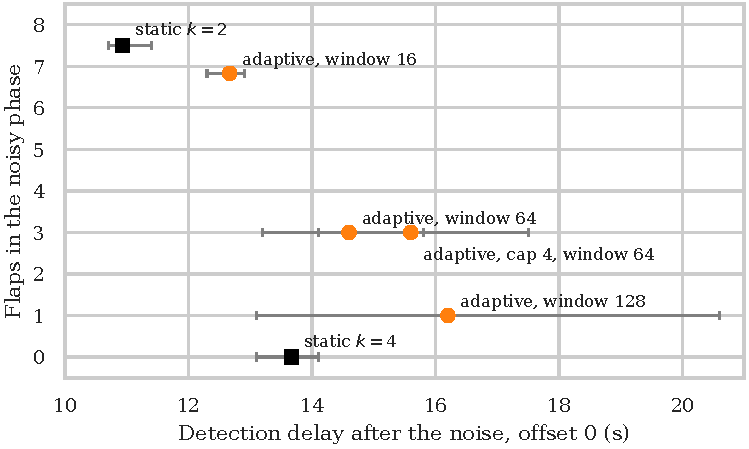
\includegraphics[width=0.8\linewidth]{figures/figure_live_tradeoff.pdf}
\caption{Flaps against detection delay in the live three-phase runs. Squares are
static thresholds, circles the adaptive ones; the bars span the three runs at offset
0. Lower and to the left is better.}
\label{fig:live-tradeoff}
\end{figure}

A static threshold of 4 never flapped and stayed \textsc{Anchored} through the noisy
phase of all six runs, at a detection delay of 13.7\,s against 10.9\,s for $k{=}2$,
which flapped 7.5 times and spent 82\% of the phase \textsc{Anchored}. The adaptive
threshold suppressed more as its window grew, 6.8 flaps for a window of 16 blocks,
3.0 for 64 and 1.0 for 128, which is close to the simulation for windows of 16 and
64 (6.1 and 3.4 flaps). It paid for that in detection at offset 0, 12.7, 14.6 and
16.2\,s. No adaptive configuration reached the flap count of the static threshold
of 4 at a shorter delay; the only one faster than it, with a window of 16, flapped
6.8 times. After an offset of 60\,s the adaptive level had decayed: with a window of
64 the detection took 9.8\,s against 11.5\,s for the static threshold of 4, the
ranges not overlapping, though with three runs each this is an observation, not an
estimate. For $k{=}2$, a window of 16 and a window of 128 the chain left
\textsc{Anchored} before the outage in all three runs at that offset, so no
detection delay was measured; we did not identify the cause.

\textbf{Repeated trigger (live).} The live adversary stops every Celestia bridge
for a nominal pulse of 3\,s and restarts them, 21 to 23 times in about ten
minutes (15 runs, three per configuration, each on a fresh genesis). Stopping and
restarting take time: the bridges were down for 15--17\,s per pulse on average,
far longer than the nominal pulse and than any threshold, so a pulse is a full DA
outage and not the short warning-level burst of the simulation. In all 15 runs,
whatever the configuration, the chain left \textsc{Anchored} at the first pulse
(one demotion), reached \textsc{Sovereign}, and spent 0.2--2.2\% of the run in
\textsc{Anchored}. This experiment therefore does not separate the thresholds, and
it gives no live evidence that the adaptive threshold absorbs short pulses: the
simulation remains the only evidence for that case, and a live adversary needs a
fault faster than stopping a bridge to produce pulses shorter than the threshold.

\emph{Summary of the extension.} In the stationary live sweep the adaptive threshold
behaved like $k{=}2$ (8.3 flaps, 85\% uptime), and with a window of 64 blocks it
flapped 3.0 times. In the live three-phase runs the flaps fell with the window (6.8,
3.0 and 1.0 for 16, 64 and 128 blocks) at detection delays of 12.7, 14.6 and
16.2\,s, against no flap at 13.7\,s for a static threshold of 4. The live
repeated-trigger runs did not separate the thresholds, and the case the extension is
meant for, absorbing short repeated pulses, rests on the simulation alone. We
therefore treat a static threshold of 4 or more as the setting to use
(Section~\ref{sec:discussion}) and the backoff as a result that did not hold up.

\FloatBarrier
